\documentclass[1p]{elsarticle_modified}
%\bibliographystyle{elsarticle-num}

%\usepackage[colorlinks]{hyperref}
%\usepackage{abbrmath_seonhwa} %\Abb, \Ascr, \Acal ,\Abf, \Afrak
\usepackage{amsfonts}
\usepackage{amssymb}
\usepackage{amsmath}
\usepackage{amsthm}
\usepackage{scalefnt}
\usepackage{amsbsy}
\usepackage{kotex}
\usepackage{caption}
\usepackage{subfig}
\usepackage{color}
\usepackage{graphicx}
\usepackage{xcolor} %% white, black, red, green, blue, cyan, magenta, yellow
\usepackage{float}
\usepackage{setspace}
\usepackage{hyperref}

\usepackage{tikz}
\usetikzlibrary{arrows}

\usepackage{multirow}
\usepackage{array} % fixed length table
\usepackage{hhline}

%%%%%%%%%%%%%%%%%%%%%
\makeatletter
\renewcommand*\env@matrix[1][\arraystretch]{%
	\edef\arraystretch{#1}%
	\hskip -\arraycolsep
	\let\@ifnextchar\new@ifnextchar
	\array{*\c@MaxMatrixCols c}}
\makeatother %https://tex.stackexchange.com/questions/14071/how-can-i-increase-the-line-spacing-in-a-matrix
%%%%%%%%%%%%%%%

\usepackage[normalem]{ulem}

\newcommand{\msout}[1]{\ifmmode\text{\sout{\ensuremath{#1}}}\else\sout{#1}\fi}
%SOURCE: \msout is \stkout macro in https://tex.stackexchange.com/questions/20609/strikeout-in-math-mode

\newcommand{\cancel}[1]{
	\ifmmode
	{\color{red}\msout{#1}}
	\else
	{\color{red}\sout{#1}}
	\fi
}

\newcommand{\add}[1]{
	{\color{blue}\uwave{#1}}
}

\newcommand{\replace}[2]{
	\ifmmode
	{\color{red}\msout{#1}}{\color{blue}\uwave{#2}}
	\else
	{\color{red}\sout{#1}}{\color{blue}\uwave{#2}}
	\fi
}

\newcommand{\Sol}{\mathcal{S}} %segment
\newcommand{\D}{D} %diagram
\newcommand{\A}{\mathcal{A}} %arc


%%%%%%%%%%%%%%%%%%%%%%%%%%%%%5 test

\def\sl{\operatorname{\textup{SL}}(2,\Cbb)}
\def\psl{\operatorname{\textup{PSL}}(2,\Cbb)}
\def\quan{\mkern 1mu \triangleright \mkern 1mu}

\theoremstyle{definition}
\newtheorem{thm}{Theorem}[section]
\newtheorem{prop}[thm]{Proposition}
\newtheorem{lem}[thm]{Lemma}
\newtheorem{ques}[thm]{Question}
\newtheorem{cor}[thm]{Corollary}
\newtheorem{defn}[thm]{Definition}
\newtheorem{exam}[thm]{Example}
\newtheorem{rmk}[thm]{Remark}
\newtheorem{alg}[thm]{Algorithm}

\newcommand{\I}{\sqrt{-1}}
\begin{document}

%\begin{frontmatter}
%
%\title{Boundary parabolic representations of knots up to 8 crossings}
%
%%% Group authors per affiliation:
%\author{Yunhi Cho} 
%\address{Department of Mathematics, University of Seoul, Seoul, Korea}
%\ead{yhcho@uos.ac.kr}
%
%
%\author{Seonhwa Kim} %\fnref{s_kim}}
%\address{Center for Geometry and Physics, Institute for Basic Science, Pohang, 37673, Korea}
%\ead{ryeona17@ibs.re.kr}
%
%\author{Hyuk Kim}
%\address{Department of Mathematical Sciences, Seoul National University, Seoul 08826, Korea}
%\ead{hyukkim@snu.ac.kr}
%
%\author{Seokbeom Yoon}
%\address{Department of Mathematical Sciences, Seoul National University, Seoul, 08826,  Korea}
%\ead{sbyoon15@snu.ac.kr}
%
%\begin{abstract}
%We find all boundary parabolic representation of knots up to 8 crossings.
%
%\end{abstract}
%\begin{keyword}
%    \MSC[2010] 57M25 
%\end{keyword}
%
%\end{frontmatter}

%\linenumbers
%\tableofcontents
%
\newcommand\colored[1]{\textcolor{white}{\rule[-0.35ex]{0.8em}{1.4ex}}\kern-0.8em\color{red} #1}%
%\newcommand\colored[1]{\textcolor{white}{ #1}\kern-2.17ex	\textcolor{white}{ #1}\kern-1.81ex	\textcolor{white}{ #1}\kern-2.15ex\color{red}#1	}

{\Large $\underline{11n_{43}~(K11n_{43})}$}

\setlength{\tabcolsep}{10pt}
\renewcommand{\arraystretch}{1.6}
\vspace{1cm}\begin{tabular}{m{100pt}>{\centering\arraybackslash}m{274pt}}
\multirow{5}{120pt}{
	\centering
	\includegraphics[width=112pt]{../../../GIT/diagram.site/Diagrams/png/659_11n_43.png}\\
\ \ \ A knot diagram\footnotemark}&
\allowdisplaybreaks
\textbf{Linearized knot diagam} \\
\cline{2-2}
 &
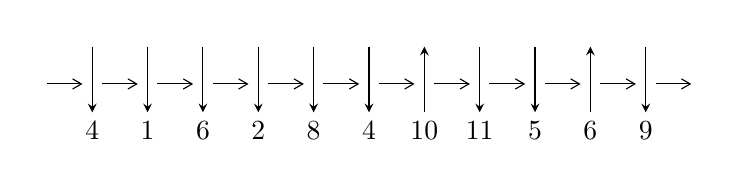
\begin{tikzpicture}[x=20pt, y=17pt]
	% nodes
	\node (C0) at (0, 0) {};
	\node (C1) at (1, 0) {};
	\node (C1U) at (1, +1) {};
	\node (C1D) at (1, -1) {4};

	\node (C2) at (2, 0) {};
	\node (C2U) at (2, +1) {};
	\node (C2D) at (2, -1) {1};

	\node (C3) at (3, 0) {};
	\node (C3U) at (3, +1) {};
	\node (C3D) at (3, -1) {6};

	\node (C4) at (4, 0) {};
	\node (C4U) at (4, +1) {};
	\node (C4D) at (4, -1) {2};

	\node (C5) at (5, 0) {};
	\node (C5U) at (5, +1) {};
	\node (C5D) at (5, -1) {8};

	\node (C6) at (6, 0) {};
	\node (C6U) at (6, +1) {};
	\node (C6D) at (6, -1) {4};

	\node (C7) at (7, 0) {};
	\node (C7U) at (7, +1) {};
	\node (C7D) at (7, -1) {10};

	\node (C8) at (8, 0) {};
	\node (C8U) at (8, +1) {};
	\node (C8D) at (8, -1) {11};

	\node (C9) at (9, 0) {};
	\node (C9U) at (9, +1) {};
	\node (C9D) at (9, -1) {5};

	\node (C10) at (10, 0) {};
	\node (C10U) at (10, +1) {};
	\node (C10D) at (10, -1) {6};

	\node (C11) at (11, 0) {};
	\node (C11U) at (11, +1) {};
	\node (C11D) at (11, -1) {9};
	\node (C12) at (12, 0) {};

	% arrows
	\draw[->,>={angle 60}]
	(C0) edge (C1) (C1) edge (C2) (C2) edge (C3) (C3) edge (C4) (C4) edge (C5) (C5) edge (C6) (C6) edge (C7) (C7) edge (C8) (C8) edge (C9) (C9) edge (C10) (C10) edge (C11) (C11) edge (C12) ;	\draw[->,>=stealth]
	(C1U) edge (C1D) (C2U) edge (C2D) (C3U) edge (C3D) (C4U) edge (C4D) (C5U) edge (C5D) (C6U) edge (C6D) (C7D) edge (C7U) (C8U) edge (C8D) (C9U) edge (C9D) (C10D) edge (C10U) (C11U) edge (C11D) ;
	\end{tikzpicture} \\
\hhline{~~} \\& 
\textbf{Solving Sequence} \\ \cline{2-2} 
 &
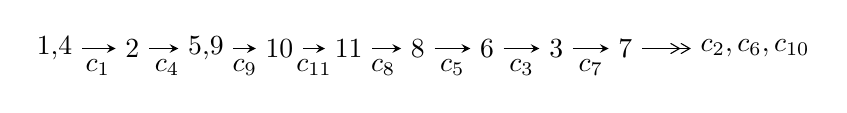
\begin{tikzpicture}[x=25pt, y=7pt]
	% node
	\node (A0) at (-1/8, 0) {1,4};
	\node (A1) at (1, 0) {2};
	\node (A2) at (33/16, 0) {5,9};
	\node (A3) at (25/8, 0) {10};
	\node (A4) at (33/8, 0) {11};
	\node (A5) at (41/8, 0) {8};
	\node (A6) at (49/8, 0) {6};
	\node (A7) at (57/8, 0) {3};
	\node (A8) at (65/8, 0) {7};
	\node (C1) at (1/2, -1) {$c_{1}$};
	\node (C2) at (3/2, -1) {$c_{4}$};
	\node (C3) at (21/8, -1) {$c_{9}$};
	\node (C4) at (29/8, -1) {$c_{11}$};
	\node (C5) at (37/8, -1) {$c_{8}$};
	\node (C6) at (45/8, -1) {$c_{5}$};
	\node (C7) at (53/8, -1) {$c_{3}$};
	\node (C8) at (61/8, -1) {$c_{7}$};
	\node (A9) at (10, 0) {$c_{2},c_{6},c_{10}$};

	% edge
	\draw[->,>=stealth]	
	(A0) edge (A1) (A1) edge (A2) (A2) edge (A3) (A3) edge (A4) (A4) edge (A5) (A5) edge (A6) (A6) edge (A7) (A7) edge (A8) ;
	\draw[->>,>={angle 60}]	
	(A8) edge (A9);
\end{tikzpicture} \\ 

\end{tabular} \\

\footnotetext{
The image of knot diagram is generated by the software ``\textbf{Draw programme}" developed by Andrew Bartholomew(\url{http://www.layer8.co.uk/maths/draw/index.htm\#Running-draw}), where we modified some parts for our purpose(\url{https://github.com/CATsTAILs/LinksPainter}).
}\phantom \\ \newline 
\centering \textbf{Ideals for irreducible components\footnotemark of $X_{\text{par}}$} 
 
\begin{align*}
I^u_{1}&=\langle 
-1.30032\times10^{39} u^{50}-9.01961\times10^{39} u^{49}+\cdots+8.75756\times10^{39} b-1.79658\times10^{40},\\
\phantom{I^u_{1}}&\phantom{= \langle  }-1.18855\times10^{39} u^{50}-7.86992\times10^{39} u^{49}+\cdots+5.47347\times10^{38} a+1.25534\times10^{39},\\
\phantom{I^u_{1}}&\phantom{= \langle  }u^{51}+7 u^{50}+\cdots-81 u^2+1\rangle \\
I^u_{2}&=\langle 
b^5- b^4-2 b^3+b^2+b+1,\;a-1,\;u-1\rangle \\
I^u_{3}&=\langle 
b+1,\;a-4 u-6,\;u^2+u-1\rangle \\
\\
\end{align*}
\raggedright * 3 irreducible components of $\dim_{\mathbb{C}}=0$, with total 58 representations.\\
\footnotetext{All coefficients of polynomials are rational numbers. But the coefficients are sometimes approximated in decimal forms when there is not enough margin.}
\newpage
\renewcommand{\arraystretch}{1}
\centering \section*{I. $I^u_{1}= \langle -1.30\times10^{39} u^{50}-9.02\times10^{39} u^{49}+\cdots+8.76\times10^{39} b-1.80\times10^{40},\;-1.19\times10^{39} u^{50}-7.87\times10^{39} u^{49}+\cdots+5.47\times10^{38} a+1.26\times10^{39},\;u^{51}+7 u^{50}+\cdots-81 u^2+1 \rangle$}
\flushleft \textbf{(i) Arc colorings}\\
\begin{tabular}{m{7pt} m{180pt} m{7pt} m{180pt} }
\flushright $a_{1}=$&$\begin{pmatrix}1\\0\end{pmatrix}$ \\
\flushright $a_{4}=$&$\begin{pmatrix}0\\u\end{pmatrix}$ \\
\flushright $a_{2}=$&$\begin{pmatrix}1\\u^2\end{pmatrix}$ \\
\flushright $a_{5}=$&$\begin{pmatrix}- u\\- u^3+u\end{pmatrix}$ \\
\flushright $a_{9}=$&$\begin{pmatrix}2.17147 u^{50}+14.3783 u^{49}+\cdots-92.5347 u-2.29349\\0.148479 u^{50}+1.02992 u^{49}+\cdots-2.01156 u+2.05146\end{pmatrix}$ \\
\flushright $a_{10}=$&$\begin{pmatrix}1.09719 u^{50}+7.70594 u^{49}+\cdots-90.5056 u-3.24898\\1.25327 u^{50}+6.81713 u^{49}+\cdots-2.96643 u+2.15932\end{pmatrix}$ \\
\flushright $a_{11}=$&$\begin{pmatrix}-1.96518 u^{50}-12.8342 u^{49}+\cdots+88.9231 u+7.11394\\-1.04684 u^{50}-6.52621 u^{49}+\cdots-0.236967 u-2.82088\end{pmatrix}$ \\
\flushright $a_{8}=$&$\begin{pmatrix}2.21621 u^{50}+14.3423 u^{49}+\cdots-4.63645 u+11.0109\\-0.0694094 u^{50}+0.202698 u^{49}+\cdots-9.54759 u+1.43747\end{pmatrix}$ \\
\flushright $a_{6}=$&$\begin{pmatrix}-0.109838 u^{50}+0.455800 u^{49}+\cdots-35.3698 u+2.83830\\2.10336 u^{50}+11.3955 u^{49}+\cdots-4.83182 u+1.99352\end{pmatrix}$ \\
\flushright $a_{3}=$&$\begin{pmatrix}- u^2+1\\u^2\end{pmatrix}$ \\
\flushright $a_{7}=$&$\begin{pmatrix}-0.109838 u^{50}+0.455800 u^{49}+\cdots-35.3698 u+2.83830\\1.41865 u^{50}+6.00756 u^{49}+\cdots-4.72198 u+0.768857\end{pmatrix}$\\ \flushright $a_{7}=$&$\begin{pmatrix}-0.109838 u^{50}+0.455800 u^{49}+\cdots-35.3698 u+2.83830\\1.41865 u^{50}+6.00756 u^{49}+\cdots-4.72198 u+0.768857\end{pmatrix}$\\&\end{tabular}
\flushleft \textbf{(ii) Obstruction class $= -1$}\\~\\
\flushleft \textbf{(iii) Cusp Shapes $= 1.81706 u^{50}+20.2990 u^{49}+\cdots-41.2566 u+8.01207$}\\~\\
\newpage\renewcommand{\arraystretch}{1}
\flushleft \textbf{(iv) u-Polynomials at the component}\newline \\
\begin{tabular}{m{50pt}|m{274pt}}
Crossings & \hspace{64pt}u-Polynomials at each crossing \\
\hline $$\begin{aligned}c_{1},c_{4}\end{aligned}$$&$\begin{aligned}
&u^{51}-7 u^{50}+\cdots+81 u^2-1
\end{aligned}$\\
\hline $$\begin{aligned}c_{2}\end{aligned}$$&$\begin{aligned}
&u^{51}+23 u^{50}+\cdots+162 u+1
\end{aligned}$\\
\hline $$\begin{aligned}c_{3},c_{6}\end{aligned}$$&$\begin{aligned}
&u^{51}-2 u^{50}+\cdots-96 u-32
\end{aligned}$\\
\hline $$\begin{aligned}c_{5}\end{aligned}$$&$\begin{aligned}
&u^{51}-3 u^{50}+\cdots+2 u-1
\end{aligned}$\\
\hline $$\begin{aligned}c_{7}\end{aligned}$$&$\begin{aligned}
&u^{51}+8 u^{50}+\cdots+64 u+4
\end{aligned}$\\
\hline $$\begin{aligned}c_{8},c_{11}\end{aligned}$$&$\begin{aligned}
&u^{51}-4 u^{50}+\cdots-87 u+1
\end{aligned}$\\
\hline $$\begin{aligned}c_{9}\end{aligned}$$&$\begin{aligned}
&u^{51}+5 u^{50}+\cdots-402 u-137
\end{aligned}$\\
\hline $$\begin{aligned}c_{10}\end{aligned}$$&$\begin{aligned}
&u^{51}+u^{50}+\cdots-4 u+31
\end{aligned}$\\
\hline
\end{tabular}\\~\\
\newpage\renewcommand{\arraystretch}{1}
\flushleft \textbf{(v) Riley Polynomials at the component}\newline \\
\begin{tabular}{m{50pt}|m{274pt}}
Crossings & \hspace{64pt}Riley Polynomials at each crossing \\
\hline $$\begin{aligned}c_{1},c_{4}\end{aligned}$$&$\begin{aligned}
&y^{51}-23 y^{50}+\cdots+162 y-1
\end{aligned}$\\
\hline $$\begin{aligned}c_{2}\end{aligned}$$&$\begin{aligned}
&y^{51}+17 y^{50}+\cdots+12790 y-1
\end{aligned}$\\
\hline $$\begin{aligned}c_{3},c_{6}\end{aligned}$$&$\begin{aligned}
&y^{51}+30 y^{50}+\cdots-8704 y-1024
\end{aligned}$\\
\hline $$\begin{aligned}c_{5}\end{aligned}$$&$\begin{aligned}
&y^{51}-15 y^{50}+\cdots+20 y-1
\end{aligned}$\\
\hline $$\begin{aligned}c_{7}\end{aligned}$$&$\begin{aligned}
&y^{51}-12 y^{50}+\cdots+1272 y-16
\end{aligned}$\\
\hline $$\begin{aligned}c_{8},c_{11}\end{aligned}$$&$\begin{aligned}
&y^{51}-30 y^{50}+\cdots+6683 y-1
\end{aligned}$\\
\hline $$\begin{aligned}c_{9}\end{aligned}$$&$\begin{aligned}
&y^{51}+37 y^{50}+\cdots+211472 y-18769
\end{aligned}$\\
\hline $$\begin{aligned}c_{10}\end{aligned}$$&$\begin{aligned}
&y^{51}+29 y^{50}+\cdots+22708 y-961
\end{aligned}$\\
\hline
\end{tabular}\\~\\
\newpage\flushleft \textbf{(vi) Complex Volumes and Cusp Shapes}
$$\begin{array}{c|c|c}  
\text{Solutions to }I^u_{1}& \I (\text{vol} + \sqrt{-1}CS) & \text{Cusp shape}\\
 \hline 
\begin{aligned}
u &= \phantom{-}0.923570 + 0.305757 I \\
a &= -0.56446 - 2.60605 I \\
b &= \phantom{-}1.108610 + 0.499436 I\end{aligned}
 & -3.69039 - 2.13393 I & -15.8264 + 4.5625 I \\ \hline\begin{aligned}
u &= \phantom{-}0.923570 - 0.305757 I \\
a &= -0.56446 + 2.60605 I \\
b &= \phantom{-}1.108610 - 0.499436 I\end{aligned}
 & -3.69039 + 2.13393 I & -15.8264 - 4.5625 I \\ \hline\begin{aligned}
u &= -0.359247 + 0.982542 I \\
a &= \phantom{-}0.110085 + 0.563683 I \\
b &= -0.885970 - 0.593352 I\end{aligned}
 & \phantom{-}4.54085 - 1.95941 I & -3.52747 + 2.51429 I \\ \hline\begin{aligned}
u &= -0.359247 - 0.982542 I \\
a &= \phantom{-}0.110085 - 0.563683 I \\
b &= -0.885970 + 0.593352 I\end{aligned}
 & \phantom{-}4.54085 + 1.95941 I & -3.52747 - 2.51429 I \\ \hline\begin{aligned}
u &= -0.872616 + 0.581002 I \\
a &= \phantom{-}0.200453 + 0.860825 I \\
b &= \phantom{-}1.74486 + 0.17305 I\end{aligned}
 & -2.26568 + 2.29719 I & -12.40272 - 3.03914 I \\ \hline\begin{aligned}
u &= -0.872616 - 0.581002 I \\
a &= \phantom{-}0.200453 - 0.860825 I \\
b &= \phantom{-}1.74486 - 0.17305 I\end{aligned}
 & -2.26568 - 2.29719 I & -12.40272 + 3.03914 I \\ \hline\begin{aligned}
u &= -0.788139 + 0.707702 I \\
a &= -0.197062 - 1.246490 I \\
b &= \phantom{-}0.879652 + 0.299225 I\end{aligned}
 & \phantom{-}1.43007 + 1.84298 I & -7.00000 - 8.98031 I \\ \hline\begin{aligned}
u &= -0.788139 - 0.707702 I \\
a &= -0.197062 + 1.246490 I \\
b &= \phantom{-}0.879652 - 0.299225 I\end{aligned}
 & \phantom{-}1.43007 - 1.84298 I & -7.00000 + 8.98031 I \\ \hline\begin{aligned}
u &= \phantom{-}0.744937 + 0.557874 I \\
a &= \phantom{-}0.337383 - 1.321850 I \\
b &= -0.203100 + 0.865788 I\end{aligned}
 & \phantom{-}0.62734 - 3.24727 I & -5.87868 + 5.45997 I \\ \hline\begin{aligned}
u &= \phantom{-}0.744937 - 0.557874 I \\
a &= \phantom{-}0.337383 + 1.321850 I \\
b &= -0.203100 - 0.865788 I\end{aligned}
 & \phantom{-}0.62734 + 3.24727 I & -5.87868 - 5.45997 I\\
 \hline 
 \end{array}$$\newpage$$\begin{array}{c|c|c}  
\text{Solutions to }I^u_{1}& \I (\text{vol} + \sqrt{-1}CS) & \text{Cusp shape}\\
 \hline 
\begin{aligned}
u &= \phantom{-}1.073300 + 0.130259 I \\
a &= -0.350884 - 1.323440 I \\
b &= \phantom{-}1.192740 - 0.253796 I\end{aligned}
 & -4.21875 + 0.45905 I & -12.7704 - 7.0072 I \\ \hline\begin{aligned}
u &= \phantom{-}1.073300 - 0.130259 I \\
a &= -0.350884 + 1.323440 I \\
b &= \phantom{-}1.192740 + 0.253796 I\end{aligned}
 & -4.21875 - 0.45905 I & -12.7704 + 7.0072 I \\ \hline\begin{aligned}
u &= -0.665417 + 0.633317 I \\
a &= -0.891675 - 0.347330 I \\
b &= \phantom{-}0.946736 + 0.983782 I\end{aligned}
 & \phantom{-}0.08535 - 1.42859 I & -8.20291 + 2.86015 I \\ \hline\begin{aligned}
u &= -0.665417 - 0.633317 I \\
a &= -0.891675 + 0.347330 I \\
b &= \phantom{-}0.946736 - 0.983782 I\end{aligned}
 & \phantom{-}0.08535 + 1.42859 I & -8.20291 - 2.86015 I \\ \hline\begin{aligned}
u &= -0.603362 + 0.919845 I \\
a &= -0.417893 - 1.298460 I \\
b &= -0.357813 + 1.171210 I\end{aligned}
 & \phantom{-}6.12236 - 2.89222 I & -7.00000 + 0. I\phantom{ +0.000000I} \\ \hline\begin{aligned}
u &= -0.603362 - 0.919845 I \\
a &= -0.417893 + 1.298460 I \\
b &= -0.357813 - 1.171210 I\end{aligned}
 & \phantom{-}6.12236 + 2.89222 I & -7.00000 + 0. I\phantom{ +0.000000I} \\ \hline\begin{aligned}
u &= \phantom{-}0.709519 + 0.862840 I \\
a &= \phantom{-}0.722213 - 0.172154 I \\
b &= -0.978955 + 0.420067 I\end{aligned}
 & -1.46329 + 2.48395 I & \phantom{-0.000000 } 0 \\ \hline\begin{aligned}
u &= \phantom{-}0.709519 - 0.862840 I \\
a &= \phantom{-}0.722213 + 0.172154 I \\
b &= -0.978955 - 0.420067 I\end{aligned}
 & -1.46329 - 2.48395 I & \phantom{-0.000000 } 0 \\ \hline\begin{aligned}
u &= -0.923670 + 0.689242 I \\
a &= \phantom{-}1.03818 + 2.23313 I \\
b &= \phantom{-}1.060170 - 0.222360 I\end{aligned}
 & \phantom{-}1.01385 + 3.52246 I & \phantom{-0.000000 } 0 \\ \hline\begin{aligned}
u &= -0.923670 - 0.689242 I \\
a &= \phantom{-}1.03818 - 2.23313 I \\
b &= \phantom{-}1.060170 + 0.222360 I\end{aligned}
 & \phantom{-}1.01385 - 3.52246 I & \phantom{-0.000000 } 0\\
 \hline 
 \end{array}$$\newpage$$\begin{array}{c|c|c}  
\text{Solutions to }I^u_{1}& \I (\text{vol} + \sqrt{-1}CS) & \text{Cusp shape}\\
 \hline 
\begin{aligned}
u &= -0.437529 + 1.071430 I \\
a &= \phantom{-}0.555165 + 0.712106 I \\
b &= -1.24641 - 0.67694 I\end{aligned}
 & \phantom{-}3.27749 - 9.36362 I & \phantom{-0.000000 } 0 \\ \hline\begin{aligned}
u &= -0.437529 - 1.071430 I \\
a &= \phantom{-}0.555165 - 0.712106 I \\
b &= -1.24641 + 0.67694 I\end{aligned}
 & \phantom{-}3.27749 + 9.36362 I & \phantom{-0.000000 } 0 \\ \hline\begin{aligned}
u &= -0.834183 + 0.022964 I \\
a &= -1.240400 - 0.071253 I \\
b &= -1.46648 - 0.21508 I\end{aligned}
 & -7.16136 - 4.34566 I & \phantom{-}0.37647 + 1.57270 I \\ \hline\begin{aligned}
u &= -0.834183 - 0.022964 I \\
a &= -1.240400 + 0.071253 I \\
b &= -1.46648 + 0.21508 I\end{aligned}
 & -7.16136 + 4.34566 I & \phantom{-}0.37647 - 1.57270 I \\ \hline\begin{aligned}
u &= \phantom{-}1.051020 + 0.519122 I \\
a &= -0.876858 + 0.965223 I \\
b &= -0.593255 - 0.386139 I\end{aligned}
 & -0.294650 - 1.061440 I & \phantom{-0.000000 } 0 \\ \hline\begin{aligned}
u &= \phantom{-}1.051020 - 0.519122 I \\
a &= -0.876858 - 0.965223 I \\
b &= -0.593255 + 0.386139 I\end{aligned}
 & -0.294650 + 1.061440 I & \phantom{-0.000000 } 0 \\ \hline\begin{aligned}
u &= -0.993259 + 0.639230 I \\
a &= \phantom{-}0.50831 + 1.57361 I \\
b &= \phantom{-}1.30081 - 0.93720 I\end{aligned}
 & -0.91339 + 6.46505 I & \phantom{-0.000000 } 0 \\ \hline\begin{aligned}
u &= -0.993259 - 0.639230 I \\
a &= \phantom{-}0.50831 - 1.57361 I \\
b &= \phantom{-}1.30081 + 0.93720 I\end{aligned}
 & -0.91339 - 6.46505 I & \phantom{-0.000000 } 0 \\ \hline\begin{aligned}
u &= \phantom{-}1.222940 + 0.084782 I \\
a &= -0.880621 + 0.184837 I \\
b &= -0.175938 + 0.530024 I\end{aligned}
 & -1.13007 - 1.28368 I & \phantom{-0.000000 } 0 \\ \hline\begin{aligned}
u &= \phantom{-}1.222940 - 0.084782 I \\
a &= -0.880621 - 0.184837 I \\
b &= -0.175938 - 0.530024 I\end{aligned}
 & -1.13007 + 1.28368 I & \phantom{-0.000000 } 0\\
 \hline 
 \end{array}$$\newpage$$\begin{array}{c|c|c}  
\text{Solutions to }I^u_{1}& \I (\text{vol} + \sqrt{-1}CS) & \text{Cusp shape}\\
 \hline 
\begin{aligned}
u &= -0.719478 + 1.003150 I \\
a &= -0.078844 - 0.785446 I \\
b &= -0.623365 + 0.588618 I\end{aligned}
 & \phantom{-}5.28316 + 2.70789 I & \phantom{-0.000000 } 0 \\ \hline\begin{aligned}
u &= -0.719478 - 1.003150 I \\
a &= -0.078844 + 0.785446 I \\
b &= -0.623365 - 0.588618 I\end{aligned}
 & \phantom{-}5.28316 - 2.70789 I & \phantom{-0.000000 } 0 \\ \hline\begin{aligned}
u &= \phantom{-}0.990585 + 0.737126 I \\
a &= \phantom{-}0.01937 + 1.54321 I \\
b &= -1.190760 - 0.548951 I\end{aligned}
 & -2.32039 - 8.39966 I & \phantom{-0.000000 } 0 \\ \hline\begin{aligned}
u &= \phantom{-}0.990585 - 0.737126 I \\
a &= \phantom{-}0.01937 - 1.54321 I \\
b &= -1.190760 + 0.548951 I\end{aligned}
 & -2.32039 + 8.39966 I & \phantom{-0.000000 } 0 \\ \hline\begin{aligned}
u &= \phantom{-}0.742417 + 0.124155 I \\
a &= -3.86813 - 7.11674 I \\
b &= \phantom{-}0.960382 - 0.003997 I\end{aligned}
 & -2.64938 - 0.11132 I & -58.9394 + 3.8883 I \\ \hline\begin{aligned}
u &= \phantom{-}0.742417 - 0.124155 I \\
a &= -3.86813 + 7.11674 I \\
b &= \phantom{-}0.960382 + 0.003997 I\end{aligned}
 & -2.64938 + 0.11132 I & -58.9394 - 3.8883 I \\ \hline\begin{aligned}
u &= -1.086370 + 0.734156 I \\
a &= \phantom{-}0.744054 + 0.739625 I \\
b &= -0.176246 - 1.311490 I\end{aligned}
 & \phantom{-}4.63878 + 8.97661 I & \phantom{-0.000000 } 0 \\ \hline\begin{aligned}
u &= -1.086370 - 0.734156 I \\
a &= \phantom{-}0.744054 - 0.739625 I \\
b &= -0.176246 + 1.311490 I\end{aligned}
 & \phantom{-}4.63878 - 8.97661 I & \phantom{-0.000000 } 0 \\ \hline\begin{aligned}
u &= -1.035770 + 0.809017 I \\
a &= \phantom{-}0.136581 + 0.365352 I \\
b &= -0.281742 - 0.574694 I\end{aligned}
 & \phantom{-}4.27954 + 3.84215 I & \phantom{-0.000000 } 0 \\ \hline\begin{aligned}
u &= -1.035770 - 0.809017 I \\
a &= \phantom{-}0.136581 - 0.365352 I \\
b &= -0.281742 + 0.574694 I\end{aligned}
 & \phantom{-}4.27954 - 3.84215 I & \phantom{-0.000000 } 0\\
 \hline 
 \end{array}$$\newpage$$\begin{array}{c|c|c}  
\text{Solutions to }I^u_{1}& \I (\text{vol} + \sqrt{-1}CS) & \text{Cusp shape}\\
 \hline 
\begin{aligned}
u &= \phantom{-}0.650449\phantom{ +0.000000I} \\
a &= -0.858462\phantom{ +0.000000I} \\
b &= -0.0122379\phantom{ +0.000000I}\end{aligned}
 & -1.00288\phantom{ +0.000000I} & -10.0670\phantom{ +0.000000I} \\ \hline\begin{aligned}
u &= -1.227370 + 0.667999 I \\
a &= -0.673896 - 1.098580 I \\
b &= -1.113660 + 0.462367 I\end{aligned}
 & \phantom{-}1.87901 + 7.98783 I & \phantom{-0.000000 } 0 \\ \hline\begin{aligned}
u &= -1.227370 - 0.667999 I \\
a &= -0.673896 + 1.098580 I \\
b &= -1.113660 - 0.462367 I\end{aligned}
 & \phantom{-}1.87901 - 7.98783 I & \phantom{-0.000000 } 0 \\ \hline\begin{aligned}
u &= -1.213470 + 0.718395 I \\
a &= -0.57099 - 1.54335 I \\
b &= -1.36456 + 0.66315 I\end{aligned}
 & \phantom{-}0.8642 + 15.7945 I & \phantom{-0.000000 } 0 \\ \hline\begin{aligned}
u &= -1.213470 - 0.718395 I \\
a &= -0.57099 + 1.54335 I \\
b &= -1.36456 - 0.66315 I\end{aligned}
 & \phantom{-}0.8642 - 15.7945 I & \phantom{-0.000000 } 0 \\ \hline\begin{aligned}
u &= \phantom{-}1.46886 + 0.10563 I \\
a &= -0.596843 + 0.030342 I \\
b &= -1.121090 + 0.463770 I\end{aligned}
 & -3.74009 + 5.32281 I & \phantom{-0.000000 } 0 \\ \hline\begin{aligned}
u &= \phantom{-}1.46886 - 0.10563 I \\
a &= -0.596843 - 0.030342 I \\
b &= -1.121090 - 0.463770 I\end{aligned}
 & -3.74009 - 5.32281 I & \phantom{-0.000000 } 0 \\ \hline\begin{aligned}
u &= -1.64237\phantom{ +0.000000I} \\
a &= -0.478176\phantom{ +0.000000I} \\
b &= -0.962556\phantom{ +0.000000I}\end{aligned}
 & -10.4502\phantom{ +0.000000I} & \phantom{-0.000000 } 0 \\ \hline\begin{aligned}
u &= -0.218706 + 0.056088 I \\
a &= -0.19747 + 1.88909 I \\
b &= \phantom{-}0.500772 + 0.518382 I\end{aligned}
 & -0.61038 - 1.48999 I & -4.46560 + 4.54978 I \\ \hline\begin{aligned}
u &= -0.218706 - 0.056088 I \\
a &= -0.19747 - 1.88909 I \\
b &= \phantom{-}0.500772 - 0.518382 I\end{aligned}
 & -0.61038 + 1.48999 I & -4.46560 - 4.54978 I\\
 \hline 
 \end{array}$$\newpage$$\begin{array}{c|c|c}  
\text{Solutions to }I^u_{1}& \I (\text{vol} + \sqrt{-1}CS) & \text{Cusp shape}\\
 \hline 
\begin{aligned}
u &= \phantom{-}0.0948151\phantom{ +0.000000I} \\
a &= -15.5949\phantom{ +0.000000I} \\
b &= \phantom{-}1.14404\phantom{ +0.000000I}\end{aligned}
 & -2.29513\phantom{ +0.000000I} & -1.15090\phantom{ +0.000000I}\\
 \hline 
 \end{array}$$\newpage\newpage\renewcommand{\arraystretch}{1}
\centering \section*{II. $I^u_{2}= \langle b^5- b^4-2 b^3+b^2+b+1,\;a-1,\;u-1 \rangle$}
\flushleft \textbf{(i) Arc colorings}\\
\begin{tabular}{m{7pt} m{180pt} m{7pt} m{180pt} }
\flushright $a_{1}=$&$\begin{pmatrix}1\\0\end{pmatrix}$ \\
\flushright $a_{4}=$&$\begin{pmatrix}0\\1\end{pmatrix}$ \\
\flushright $a_{2}=$&$\begin{pmatrix}1\\1\end{pmatrix}$ \\
\flushright $a_{5}=$&$\begin{pmatrix}-1\\0\end{pmatrix}$ \\
\flushright $a_{9}=$&$\begin{pmatrix}1\\b\end{pmatrix}$ \\
\flushright $a_{10}=$&$\begin{pmatrix}- b+1\\b\end{pmatrix}$ \\
\flushright $a_{11}=$&$\begin{pmatrix}- b+1\\- b^2\end{pmatrix}$ \\
\flushright $a_{8}=$&$\begin{pmatrix}- b^2+b+1\\- b^3+b\end{pmatrix}$ \\
\flushright $a_{6}=$&$\begin{pmatrix}0\\- b^4- b^3+b^2+2 b+1\end{pmatrix}$ \\
\flushright $a_{3}=$&$\begin{pmatrix}0\\1\end{pmatrix}$ \\
\flushright $a_{7}=$&$\begin{pmatrix}0\\- b^4- b^3+b^2+2 b+1\end{pmatrix}$\\ \flushright $a_{7}=$&$\begin{pmatrix}0\\- b^4- b^3+b^2+2 b+1\end{pmatrix}$\\&\end{tabular}
\flushleft \textbf{(ii) Obstruction class $= 1$}\\~\\
\flushleft \textbf{(iii) Cusp Shapes $= 3 b^4+b^3-2 b^2-10 b-17$}\\~\\
\newpage\renewcommand{\arraystretch}{1}
\flushleft \textbf{(iv) u-Polynomials at the component}\newline \\
\begin{tabular}{m{50pt}|m{274pt}}
Crossings & \hspace{64pt}u-Polynomials at each crossing \\
\hline $$\begin{aligned}c_{1}\end{aligned}$$&$\begin{aligned}
&(u-1)^5
\end{aligned}$\\
\hline $$\begin{aligned}c_{2},c_{4}\end{aligned}$$&$\begin{aligned}
&(u+1)^5
\end{aligned}$\\
\hline $$\begin{aligned}c_{3},c_{6}\end{aligned}$$&$\begin{aligned}
&u^5
\end{aligned}$\\
\hline $$\begin{aligned}c_{5}\end{aligned}$$&$\begin{aligned}
&u^5-3 u^4+4 u^3- u^2- u+1
\end{aligned}$\\
\hline $$\begin{aligned}c_{7}\end{aligned}$$&$\begin{aligned}
&u^5- u^4+2 u^3- u^2+u-1
\end{aligned}$\\
\hline $$\begin{aligned}c_{8}\end{aligned}$$&$\begin{aligned}
&u^5+u^4-2 u^3- u^2+u-1
\end{aligned}$\\
\hline $$\begin{aligned}c_{9},c_{11}\end{aligned}$$&$\begin{aligned}
&u^5- u^4-2 u^3+u^2+u+1
\end{aligned}$\\
\hline $$\begin{aligned}c_{10}\end{aligned}$$&$\begin{aligned}
&u^5+u^4+2 u^3+u^2+u+1
\end{aligned}$\\
\hline
\end{tabular}\\~\\
\newpage\renewcommand{\arraystretch}{1}
\flushleft \textbf{(v) Riley Polynomials at the component}\newline \\
\begin{tabular}{m{50pt}|m{274pt}}
Crossings & \hspace{64pt}Riley Polynomials at each crossing \\
\hline $$\begin{aligned}c_{1},c_{2},c_{4}\end{aligned}$$&$\begin{aligned}
&(y-1)^5
\end{aligned}$\\
\hline $$\begin{aligned}c_{3},c_{6}\end{aligned}$$&$\begin{aligned}
&y^5
\end{aligned}$\\
\hline $$\begin{aligned}c_{5}\end{aligned}$$&$\begin{aligned}
&y^5- y^4+8 y^3-3 y^2+3 y-1
\end{aligned}$\\
\hline $$\begin{aligned}c_{7},c_{10}\end{aligned}$$&$\begin{aligned}
&y^5+3 y^4+4 y^3+y^2- y-1
\end{aligned}$\\
\hline $$\begin{aligned}c_{8},c_{9},c_{11}\end{aligned}$$&$\begin{aligned}
&y^5-5 y^4+8 y^3-3 y^2- y-1
\end{aligned}$\\
\hline
\end{tabular}\\~\\
\newpage\flushleft \textbf{(vi) Complex Volumes and Cusp Shapes}
$$\begin{array}{c|c|c}  
\text{Solutions to }I^u_{2}& \I (\text{vol} + \sqrt{-1}CS) & \text{Cusp shape}\\
 \hline 
\begin{aligned}
u &= \phantom{-}1.00000\phantom{ +0.000000I} \\
a &= \phantom{-}1.00000\phantom{ +0.000000I} \\
b &= -1.21774\phantom{ +0.000000I}\end{aligned}
 & -4.04602\phantom{ +0.000000I} & -2.99730\phantom{ +0.000000I} \\ \hline\begin{aligned}
u &= \phantom{-}1.00000\phantom{ +0.000000I} \\
a &= \phantom{-}1.00000\phantom{ +0.000000I} \\
b &= -0.309916 + 0.549911 I\end{aligned}
 & -1.97403 + 1.53058 I & -13.4575 - 4.4032 I \\ \hline\begin{aligned}
u &= \phantom{-}1.00000\phantom{ +0.000000I} \\
a &= \phantom{-}1.00000\phantom{ +0.000000I} \\
b &= -0.309916 - 0.549911 I\end{aligned}
 & -1.97403 - 1.53058 I & -13.4575 + 4.4032 I \\ \hline\begin{aligned}
u &= \phantom{-}1.00000\phantom{ +0.000000I} \\
a &= \phantom{-}1.00000\phantom{ +0.000000I} \\
b &= \phantom{-}1.41878 + 0.21917 I\end{aligned}
 & -7.51750 - 4.40083 I & -22.0438 + 5.2094 I \\ \hline\begin{aligned}
u &= \phantom{-}1.00000\phantom{ +0.000000I} \\
a &= \phantom{-}1.00000\phantom{ +0.000000I} \\
b &= \phantom{-}1.41878 - 0.21917 I\end{aligned}
 & -7.51750 + 4.40083 I & -22.0438 - 5.2094 I\\
 \hline 
 \end{array}$$\newpage\newpage\renewcommand{\arraystretch}{1}
\centering \section*{III. $I^u_{3}= \langle b+1,\;a-4 u-6,\;u^2+u-1 \rangle$}
\flushleft \textbf{(i) Arc colorings}\\
\begin{tabular}{m{7pt} m{180pt} m{7pt} m{180pt} }
\flushright $a_{1}=$&$\begin{pmatrix}1\\0\end{pmatrix}$ \\
\flushright $a_{4}=$&$\begin{pmatrix}0\\u\end{pmatrix}$ \\
\flushright $a_{2}=$&$\begin{pmatrix}1\\- u+1\end{pmatrix}$ \\
\flushright $a_{5}=$&$\begin{pmatrix}- u\\- u+1\end{pmatrix}$ \\
\flushright $a_{9}=$&$\begin{pmatrix}4 u+6\\-1\end{pmatrix}$ \\
\flushright $a_{10}=$&$\begin{pmatrix}3 u+5\\0\end{pmatrix}$ \\
\flushright $a_{11}=$&$\begin{pmatrix}4 u+7\\-1\end{pmatrix}$ \\
\flushright $a_{8}=$&$\begin{pmatrix}-1\\0\end{pmatrix}$ \\
\flushright $a_{6}=$&$\begin{pmatrix}-1\\- u+1\end{pmatrix}$ \\
\flushright $a_{3}=$&$\begin{pmatrix}u\\- u+1\end{pmatrix}$ \\
\flushright $a_{7}=$&$\begin{pmatrix}-1\\0\end{pmatrix}$\\ \flushright $a_{7}=$&$\begin{pmatrix}-1\\0\end{pmatrix}$\\&\end{tabular}
\flushleft \textbf{(ii) Obstruction class $= 1$}\\~\\
\flushleft \textbf{(iii) Cusp Shapes $= -61$}\\~\\
\newpage\renewcommand{\arraystretch}{1}
\flushleft \textbf{(iv) u-Polynomials at the component}\newline \\
\begin{tabular}{m{50pt}|m{274pt}}
Crossings & \hspace{64pt}u-Polynomials at each crossing \\
\hline $$\begin{aligned}c_{1},c_{3}\end{aligned}$$&$\begin{aligned}
&u^2+u-1
\end{aligned}$\\
\hline $$\begin{aligned}c_{2}\end{aligned}$$&$\begin{aligned}
&u^2+3 u+1
\end{aligned}$\\
\hline $$\begin{aligned}c_{4},c_{6}\end{aligned}$$&$\begin{aligned}
&u^2- u-1
\end{aligned}$\\
\hline $$\begin{aligned}c_{5},c_{9},c_{10}\end{aligned}$$&$\begin{aligned}
&u^2-3 u+1
\end{aligned}$\\
\hline $$\begin{aligned}c_{7}\end{aligned}$$&$\begin{aligned}
&u^2
\end{aligned}$\\
\hline $$\begin{aligned}c_{8}\end{aligned}$$&$\begin{aligned}
&(u-1)^2
\end{aligned}$\\
\hline $$\begin{aligned}c_{11}\end{aligned}$$&$\begin{aligned}
&(u+1)^2
\end{aligned}$\\
\hline
\end{tabular}\\~\\
\newpage\renewcommand{\arraystretch}{1}
\flushleft \textbf{(v) Riley Polynomials at the component}\newline \\
\begin{tabular}{m{50pt}|m{274pt}}
Crossings & \hspace{64pt}Riley Polynomials at each crossing \\
\hline $$\begin{aligned}c_{1},c_{3},c_{4}\\c_{6}\end{aligned}$$&$\begin{aligned}
&y^2-3 y+1
\end{aligned}$\\
\hline $$\begin{aligned}c_{2},c_{5},c_{9}\\c_{10}\end{aligned}$$&$\begin{aligned}
&y^2-7 y+1
\end{aligned}$\\
\hline $$\begin{aligned}c_{7}\end{aligned}$$&$\begin{aligned}
&y^2
\end{aligned}$\\
\hline $$\begin{aligned}c_{8},c_{11}\end{aligned}$$&$\begin{aligned}
&(y-1)^2
\end{aligned}$\\
\hline
\end{tabular}\\~\\
\newpage\flushleft \textbf{(vi) Complex Volumes and Cusp Shapes}
$$\begin{array}{c|c|c}  
\text{Solutions to }I^u_{3}& \I (\text{vol} + \sqrt{-1}CS) & \text{Cusp shape}\\
 \hline 
\begin{aligned}
u &= \phantom{-}0.618034\phantom{ +0.000000I} \\
a &= \phantom{-}8.47214\phantom{ +0.000000I} \\
b &= -1.00000\phantom{ +0.000000I}\end{aligned}
 & -2.63189\phantom{ +0.000000I} & -61.0000\phantom{ +0.000000I} \\ \hline\begin{aligned}
u &= -1.61803\phantom{ +0.000000I} \\
a &= -0.472136\phantom{ +0.000000I} \\
b &= -1.00000\phantom{ +0.000000I}\end{aligned}
 & -10.5276\phantom{ +0.000000I} & -61.0000\phantom{ +0.000000I}\\
 \hline 
 \end{array}$$\newpage
\newpage\renewcommand{\arraystretch}{1}
\centering \section*{ IV. u-Polynomials}
\begin{tabular}{m{50pt}|m{274pt}}
Crossings & \hspace{64pt}u-Polynomials at each crossing \\
\hline $$\begin{aligned}c_{1}\end{aligned}$$&$\begin{aligned}
&((u-1)^5)(u^2+u-1)(u^{51}-7 u^{50}+\cdots+81 u^2-1)
\end{aligned}$\\
\hline $$\begin{aligned}c_{2}\end{aligned}$$&$\begin{aligned}
&((u+1)^5)(u^2+3 u+1)(u^{51}+23 u^{50}+\cdots+162 u+1)
\end{aligned}$\\
\hline $$\begin{aligned}c_{3}\end{aligned}$$&$\begin{aligned}
&u^5(u^2+u-1)(u^{51}-2 u^{50}+\cdots-96 u-32)
\end{aligned}$\\
\hline $$\begin{aligned}c_{4}\end{aligned}$$&$\begin{aligned}
&((u+1)^5)(u^2- u-1)(u^{51}-7 u^{50}+\cdots+81 u^2-1)
\end{aligned}$\\
\hline $$\begin{aligned}c_{5}\end{aligned}$$&$\begin{aligned}
&(u^2-3 u+1)(u^5-3 u^4+\cdots- u+1)(u^{51}-3 u^{50}+\cdots+2 u-1)
\end{aligned}$\\
\hline $$\begin{aligned}c_{6}\end{aligned}$$&$\begin{aligned}
&u^5(u^2- u-1)(u^{51}-2 u^{50}+\cdots-96 u-32)
\end{aligned}$\\
\hline $$\begin{aligned}c_{7}\end{aligned}$$&$\begin{aligned}
&u^2(u^5- u^4+\cdots+u-1)(u^{51}+8 u^{50}+\cdots+64 u+4)
\end{aligned}$\\
\hline $$\begin{aligned}c_{8}\end{aligned}$$&$\begin{aligned}
&((u-1)^2)(u^5+u^4+\cdots+u-1)(u^{51}-4 u^{50}+\cdots-87 u+1)
\end{aligned}$\\
\hline $$\begin{aligned}c_{9}\end{aligned}$$&$\begin{aligned}
&(u^2-3 u+1)(u^5- u^4+\cdots+u+1)(u^{51}+5 u^{50}+\cdots-402 u-137)
\end{aligned}$\\
\hline $$\begin{aligned}c_{10}\end{aligned}$$&$\begin{aligned}
&(u^2-3 u+1)(u^5+u^4+\cdots+u+1)(u^{51}+u^{50}+\cdots-4 u+31)
\end{aligned}$\\
\hline $$\begin{aligned}c_{11}\end{aligned}$$&$\begin{aligned}
&((u+1)^2)(u^5- u^4+\cdots+u+1)(u^{51}-4 u^{50}+\cdots-87 u+1)
\end{aligned}$\\
\hline
\end{tabular}\newpage\renewcommand{\arraystretch}{1}
\centering \section*{ V. Riley Polynomials}
\begin{tabular}{m{50pt}|m{274pt}}
Crossings & \hspace{64pt}Riley Polynomials at each crossing \\
\hline $$\begin{aligned}c_{1},c_{4}\end{aligned}$$&$\begin{aligned}
&((y-1)^5)(y^2-3 y+1)(y^{51}-23 y^{50}+\cdots+162 y-1)
\end{aligned}$\\
\hline $$\begin{aligned}c_{2}\end{aligned}$$&$\begin{aligned}
&((y-1)^5)(y^2-7 y+1)(y^{51}+17 y^{50}+\cdots+12790 y-1)
\end{aligned}$\\
\hline $$\begin{aligned}c_{3},c_{6}\end{aligned}$$&$\begin{aligned}
&y^5(y^2-3 y+1)(y^{51}+30 y^{50}+\cdots-8704 y-1024)
\end{aligned}$\\
\hline $$\begin{aligned}c_{5}\end{aligned}$$&$\begin{aligned}
&(y^2-7 y+1)(y^5- y^4+\cdots+3 y-1)(y^{51}-15 y^{50}+\cdots+20 y-1)
\end{aligned}$\\
\hline $$\begin{aligned}c_{7}\end{aligned}$$&$\begin{aligned}
&y^2(y^5+3 y^4+\cdots- y-1)(y^{51}-12 y^{50}+\cdots+1272 y-16)
\end{aligned}$\\
\hline $$\begin{aligned}c_{8},c_{11}\end{aligned}$$&$\begin{aligned}
&((y-1)^2)(y^5-5 y^4+\cdots- y-1)(y^{51}-30 y^{50}+\cdots+6683 y-1)
\end{aligned}$\\
\hline $$\begin{aligned}c_{9}\end{aligned}$$&$\begin{aligned}
&(y^2-7 y+1)(y^5-5 y^4+8 y^3-3 y^2- y-1)\\
&\cdot(y^{51}+37 y^{50}+\cdots+211472 y-18769)
\end{aligned}$\\
\hline $$\begin{aligned}c_{10}\end{aligned}$$&$\begin{aligned}
&(y^2-7 y+1)(y^5+3 y^4+4 y^3+y^2- y-1)\\
&\cdot(y^{51}+29 y^{50}+\cdots+22708 y-961)
\end{aligned}$\\
\hline
\end{tabular}
\vskip 2pc
\end{document}